% !TEX root =  paper.tex

\begin{figure*}[t!]
	\centering
	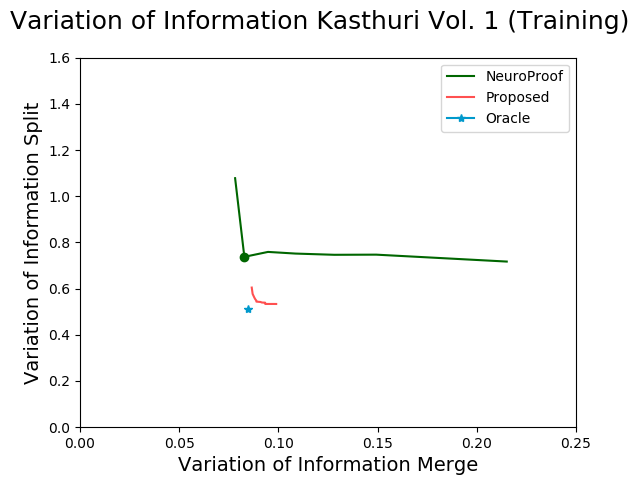
\includegraphics[width=0.45\linewidth]{./figures/variation_of_information-microns-train-600.png}
	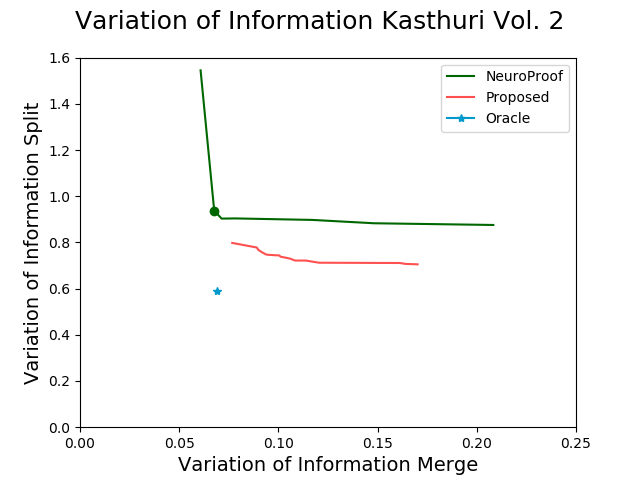
\includegraphics[width=0.45\linewidth]{./figures/variation_of_information-microns-test-600.png}
	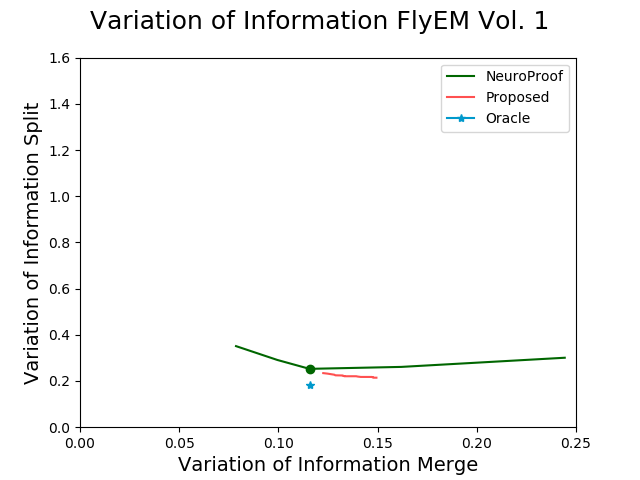
\includegraphics[width=0.45\linewidth]{./figures/variation_of_information-FlyEM-train-600.png}
	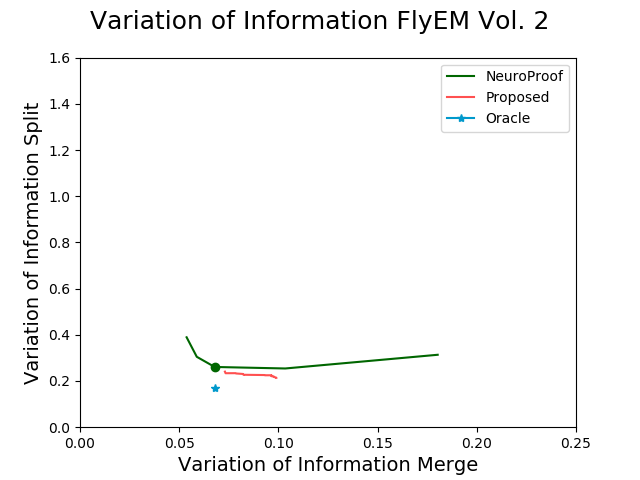
\includegraphics[width=0.45\linewidth]{./figures/variation_of_information-FlyEM-test-600.png}
	\caption{VI scores of our method (red) compared to the baseline segmentation (green) and an oracle (blue) that optimally partitions the graph based on ground truth. Lower scores are better. Our method improves the accuracy of the segmentation in all cases.}
	\label{fig:variation-of-information}
\end{figure*}

\subsection{Error Metric}
\label{sec:variation-of-information}

We evaluate the performance of the different methods using the split variation of information (VI)~\cite{meila2003comparing}.
Given a ground truth labeling $GT$ and our automatically reconstructed segmentation $SG$, over- and under-segmentation are quantified by the conditional entropies $H(GT | SG)$ and $H(SG | GT)$, respectively. 
Since we are measuring the entropy between two clusterings, lower VI scores are better.

\subsection{Variation of Information Results}

In Fig.~\ref{fig:variation-of-information}, we show the VI results of the pixel-based reconstructions of the Kasthuri and FlyEM data (Sec.~\ref{sec:neuroproof}) for varying thresholds of agglomeration (green). 
We use one of these segmentations (green circle) as our input dataset with an agglomeration threshold of 0.3 for all datasets. 
The results from our method are shown in red for varying the $\beta$ parameter. 
We show comparisons to an oracle (blue) that correctly partitions the graph from our method based on ground truth.

Our algorithm improves the accuracy of the reconstruction for every dataset, reducing the VI split score on average by \TODO{XX}\% on the three testing datasets. 
Scores closer to the origin are better for this metric, and in every instance our results are below the green curve.
We see significant improvements on the Kasthuri datasets (VI split reduction of \TODO{XX}\% and \TODO{XX}\% on the training and testing datasets respectively) and more modest improvements on the FlyEM datasets (reduction of \TODO{XX}\% and \TODO{XX}\%). 
\TODO{FIX: This is because the baseline segmentation algorithm for the isotropic FlyEM data (Sec.~\ref{sec:neuroproof}) performs much better, reducing the potential for improvements. 
Isotropic datasets are easier to segment using state-of-the-art region-based methods than anisotropic ones~\cite{plaza2014annotating}.}

Fig.~\ref{fig:qualitative-results} (left) shows successful merges on the Kasthuri Vol. 2 dataset. 
Several of these examples combine multiple consecutive segments that span the volume.
In the third example on the left we correct the over-segmentation of a dendrite and attached spine-necks.
Fig.~\ref{fig:qualitative-results} (right) shows typical failure cases of our method (red circles).
In two of these examples the algorithm correctly predicted several merges before a single error rendered the segment as wrong.
In the third example (blue circle) a merge error in the initial segmentation propagated to our output.
We now analyze how each major component of our method contributes to this final result.

\begin{figure}[t]
	\begin{minipage}{0.45\linewidth}
		\centering
		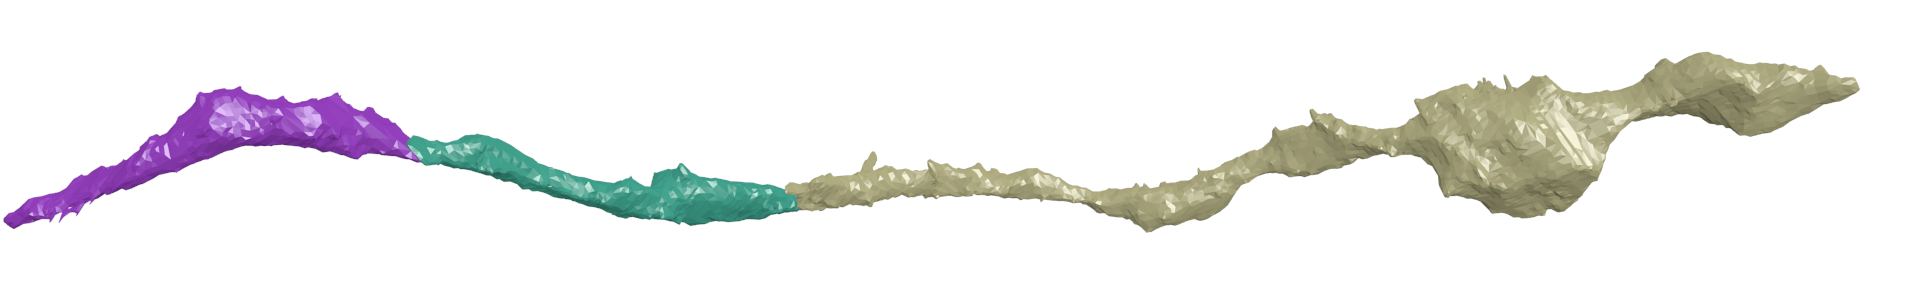
\includegraphics[width=0.85\linewidth]{./figures/VI-results/multicut-correct1.png}
		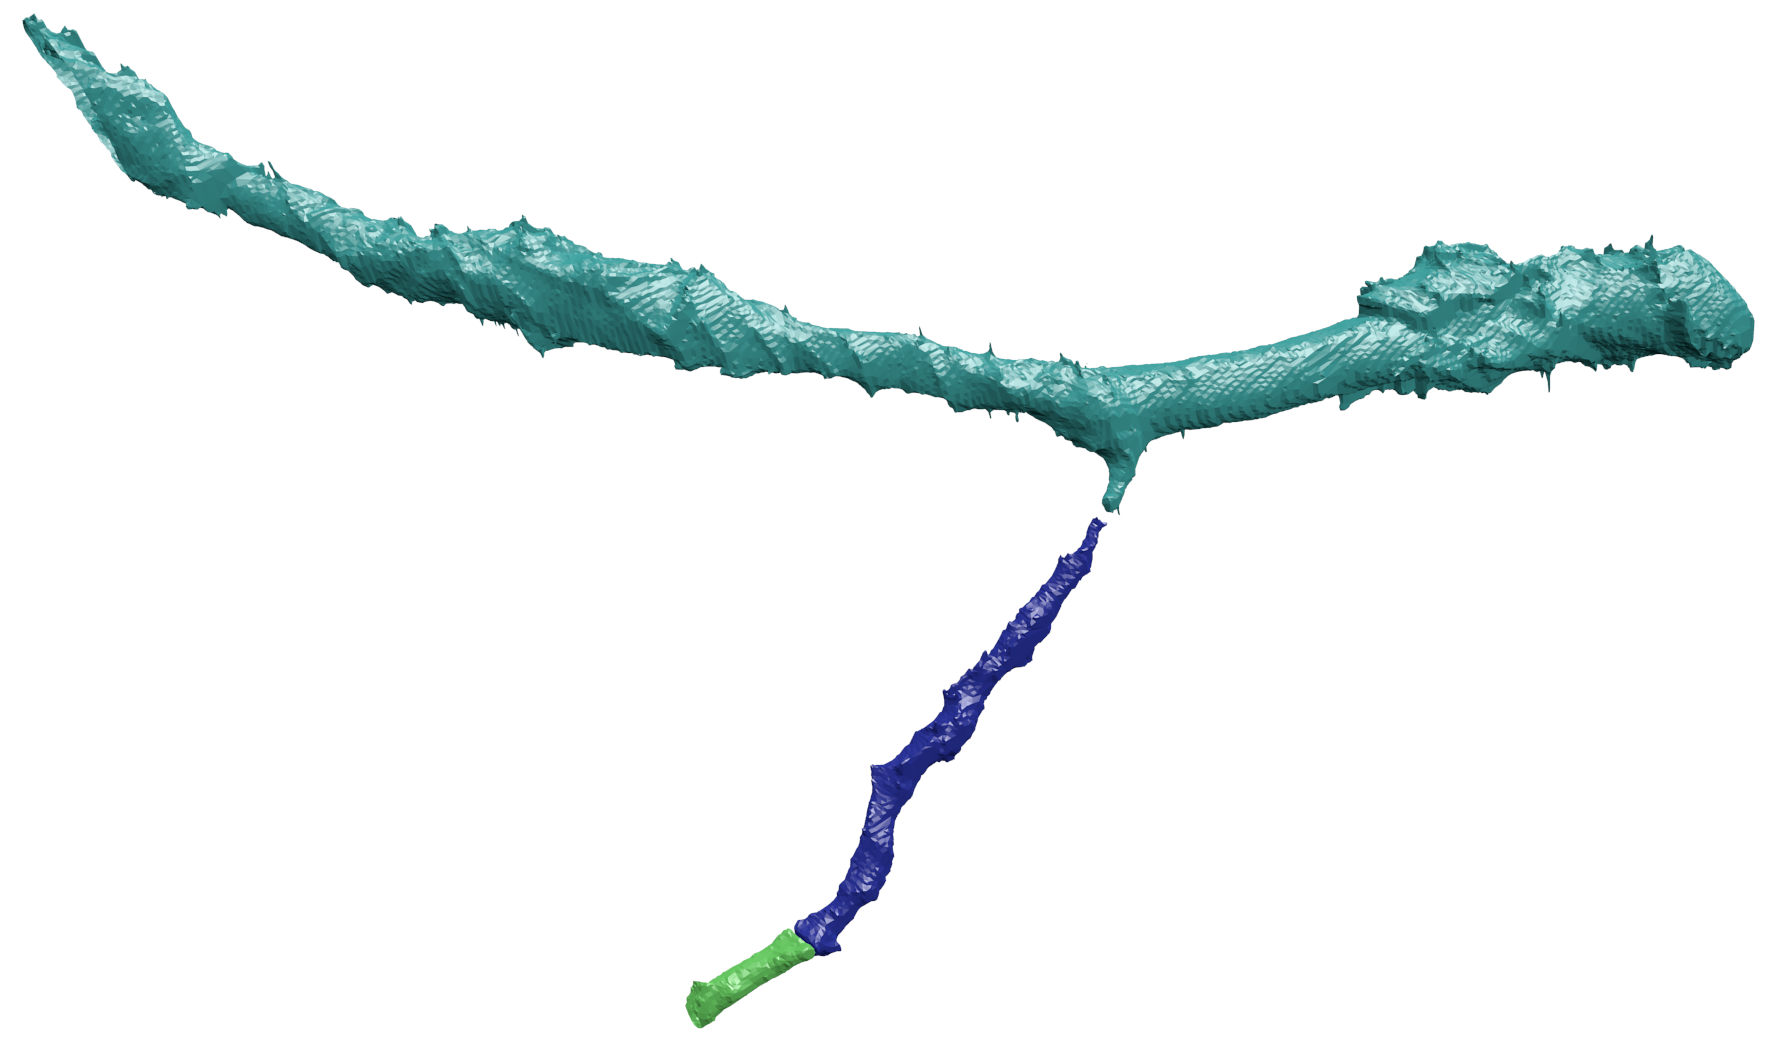
\includegraphics[width=0.85\linewidth]{./figures/VI-results/multicut-correct2.png}
		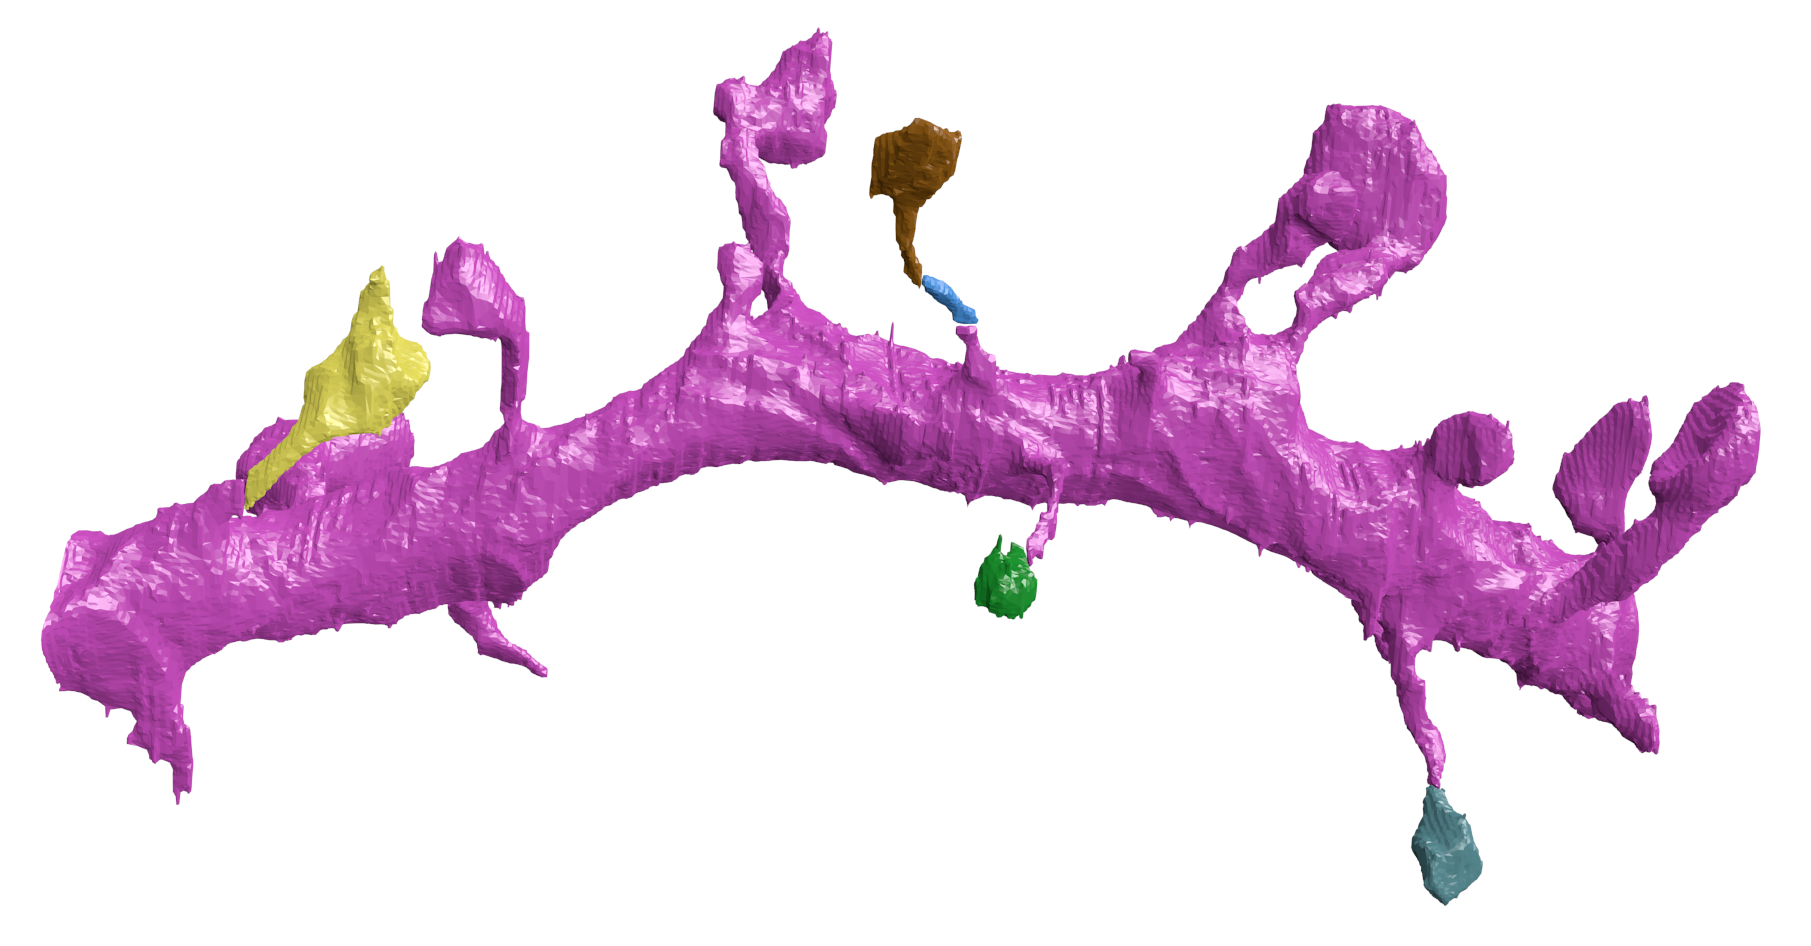
\includegraphics[width=0.85\linewidth]{./figures/VI-results/multicut-correct3.png}
		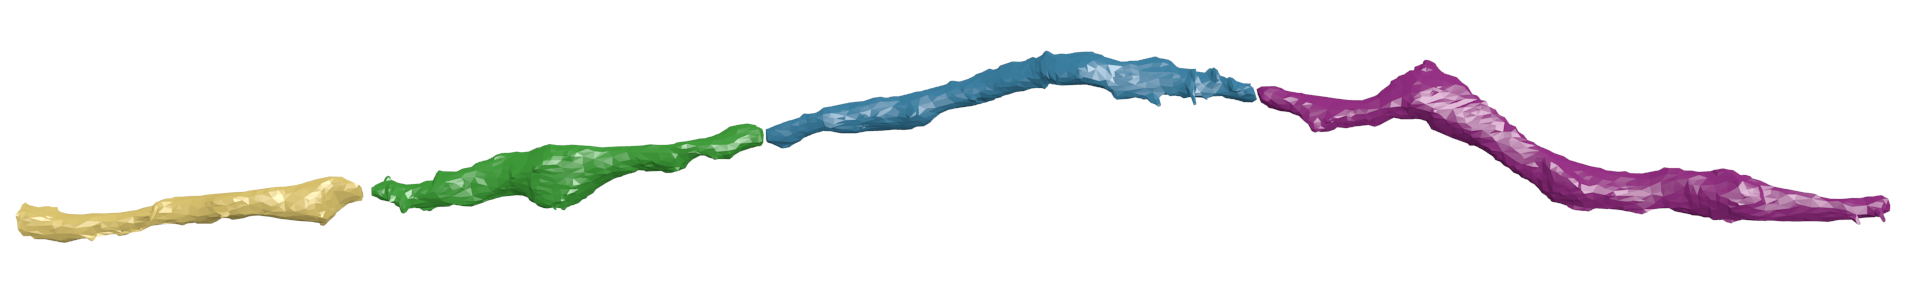
\includegraphics[width=0.85\linewidth]{./figures/VI-results/multicut-correct4.png}
		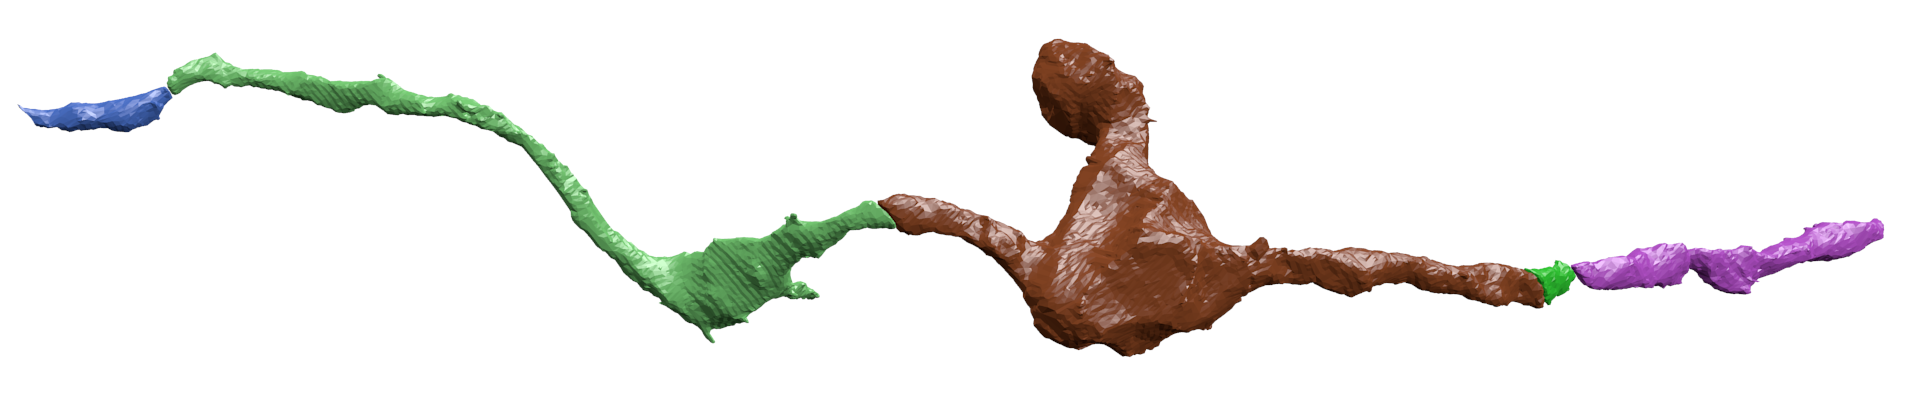
\includegraphics[width=0.85\linewidth]{./figures/VI-results/multicut-correct5.png}
	\end{minipage}
	\begin{minipage}{0.45\linewidth}
		\centering
		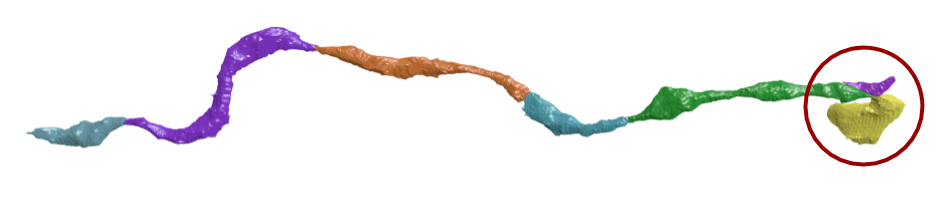
\includegraphics[width=0.85\linewidth]{./figures/VI-results/multicut-incorrect1.png}
		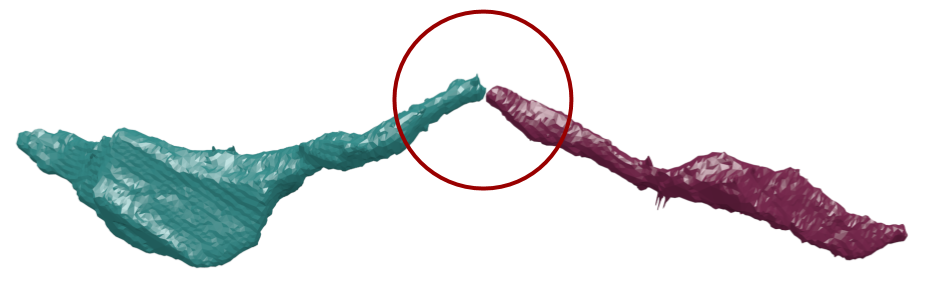
\includegraphics[width=0.85\linewidth]{./figures/VI-results/multicut-incorrect2.png}
		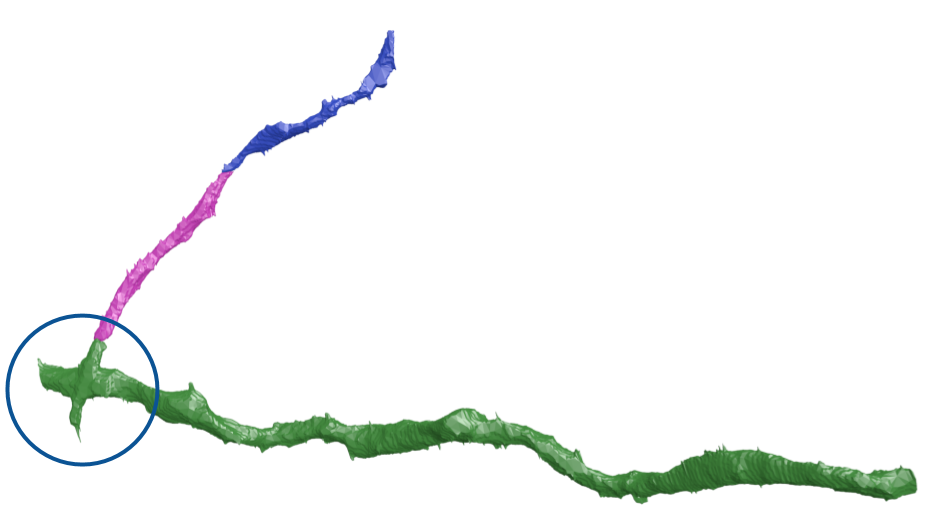
\includegraphics[width=0.85\linewidth]{./figures/VI-results/multicut-incorrect3.png}
		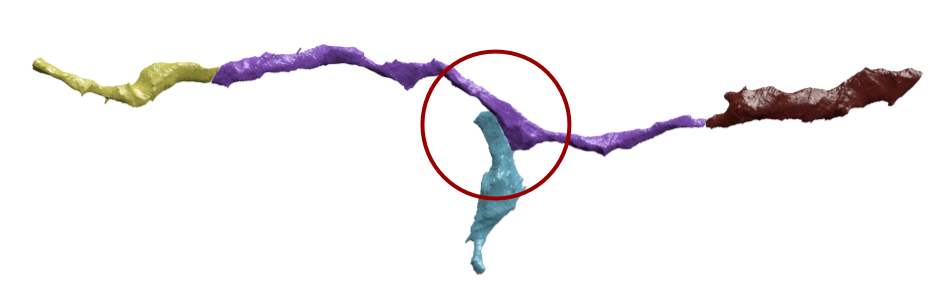
\includegraphics[width=0.85\linewidth]{./figures/VI-results/multicut-incorrect4.png}
	\end{minipage}
	\caption{(left) Segments of neurons that were correctly merged by our method. (right) Circles indicate areas of wrong merges by our method (red) or by the initial pixel-based segmentation (blue).}
	\label{fig:qualitative-results}
\end{figure}

\subsection{Graph Pruning Results}

Table \ref{table:skeletonization} shows the results of pruning the skeleton graph using the algorithm discussed in Sec.~\ref{sec:skeletonization}. 
This edge pruning is essential for the graph partitioning algorithm, which has a computational complexity dependence on the number of edges. 
The baseline algorithm considers all adjacent regions for merging. 
Our method removes a significant portion of these candidates while maintaining a large number of the true merge locations (e.g., \TODO{XXX} compared to \TODO{XXX}). 
Our pruning heuristic removes at least $\TODO{X}\times$ the number of edges on all datasets, achieving a maximum removal rate of $\TODO{XX}\times$.
However, there are some adjacent over-segmented labels which are considered. 
Table~\ref{table:skeletonization} shows the results for our edge generation including the number of missed neighbors and potential penalty in VI score.
\TODO{augment table}
We present additional analysis of the skeletonization parameters in the supplemental material.

\begin{table}
	\centering
	\small
	\begin{tabular}{c c c} \hline
		\textbf{Dataset} & \textbf{Baseline} & \textbf{After Pruning} \\ \hline
		Kasthuri Training & 763 / 21,242 & 753 / 3,459 \\
		Kasthuri Vol. 2 & 1,010 / 26,073 & 904 / 4,327 \\
		FlyEM Vol. 1 & 269 / 14,875 & 262 / 946 \\
		FlyEM Vol. 2 & 270 / 16,808 & 285 / 768 \\ \hline
		%		Kasthuri Vol. 1 & 763 / 21242 (3.47\%) & 753 / 3459 (17.88\%) \\
		%		Kasthuri Vol. 2 & 1010 / 26073 (3.73\%) & 904 / 4327 (17.28\%) \\
		%		FlyEM Vol. 1 & 269 / 14875 (1.78\%) & 262 / 946 (21.69\%) \\
		%		FlyEM Vol. 2 & 270 / 16808 (1.58\%) & 285 / 768 (27.07\%)\\ \hline
	\end{tabular}
	\caption{The results of our graph pruning approach compared to the baseline graph with all adjacent regions. We show the number of true merge locations (e.g., 763) compared to total number of edges in the graph (e.g., 21,242) for each case.}
	\label{table:skeletonization}
\end{table}

We generate edges in our graph by using information from the skeletons. 
In particular, we do not enforce the constraint that edges in our graph correspond to adjacent segments.
Although neurons are continuous, the EM images often have noisy spots which cause an interruption in the input segmentation.
We still want to reconstruct these neurons despite the fact that the initial segmentation is non-continuous. 
The second and fourth examples in Fig.~\ref{fig:qualitative-results} show correctly reconstructed neurons where two of the segments are non-adjacent. 
On average in our datasets we correctly merge \TODO{XX} number of non-adjacent segments. 

There are some pairs of segments which we do not consider for merging because of our reliance on the skeletons.
Fig.~\ref{fig:skeleton-results} shows two such cases. 
The endpoints of both segments are circled.
In this example the small segment is carved from the larger segment in a location where there are no skeleton endpoints. 
There are on average $\TODO{XX}$ such examples in our datasets, corresponding to $\TODO{XX}$ in the variation of information split score. 

\begin{figure}[t!]
	\centering
	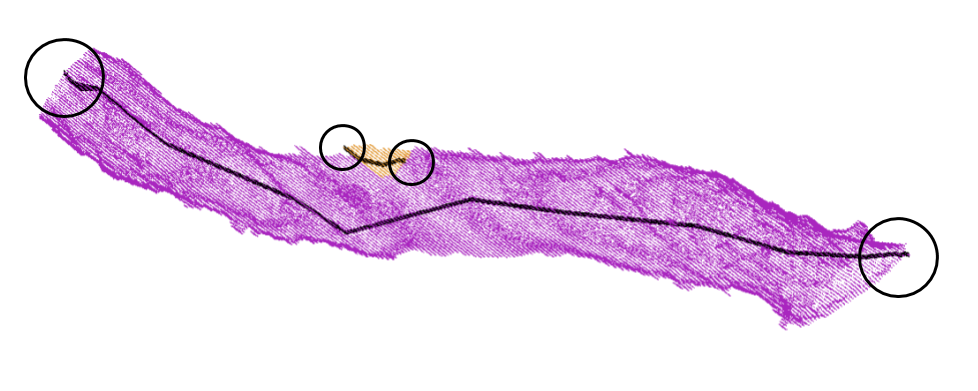
\includegraphics[width=0.45\linewidth]{./figures/merge_candidate1.png}		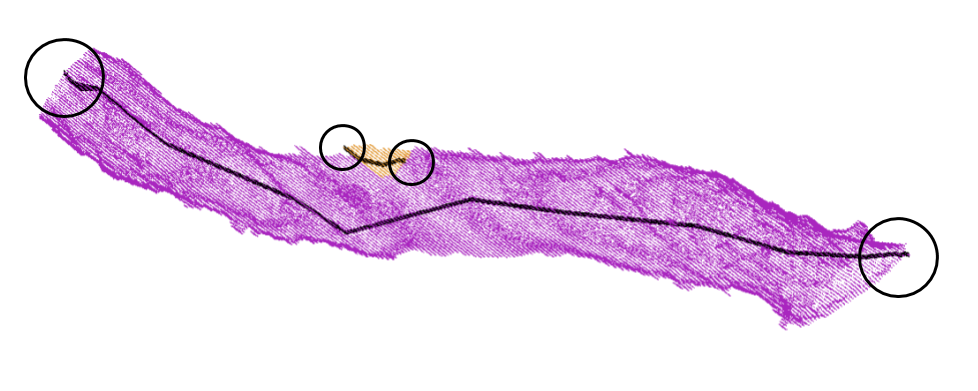
\includegraphics[width=0.45\linewidth]{./figures/merge_candidate1.png}
	\caption{Two false negative example of our method due to graph pruning. The distance between the endpoints (circled) of the two segments is too far to be flagged as a merge candidate. \TODO{SECOND EXAMPLE}}
	\label{fig:skeleton-results}
\end{figure}

\subsection{CNN Classification Results}

\paragraph{Inference Augmentation.}

Data augmentation at test time can improve accuracy results~\cite{zeng2017deepem3d,lee2017superhuman}.
When computing the probability to merge two segments, we input the initial segment into our CNN as well as \TODO{XX} randomly rotated and flipped examples (in the same manner as training augmentation).
This produces some additional increase in overall accuracy (Table ~\ref{table:inference-augmentation}). 
The supplemental material contains experiments showing the trade-offs between increased accuracy and runtime when using these augmentation strategies.

\begin{table}
	\begin{center}
		\begin{tabular}{c | c c c}
			Dataset & Precision & Recall & Accuracy \\ \hline
			Kasthuri & & & \\
			FlyEM Vol. 1 & & & \\
			FlyEM Vol. 2 & & & 
		\end{tabular}
		\caption{Data augmentation during test time increases the precision, recall, and accuracy of all three datasets.}
		\label{table:inference-augmentation}
	\end{center}
\end{table}

Fig.~\ref{fig:receiver-operating-characteristic} shows the receiver operating characteristic (ROC) curve of our CNN classifier for all test datasets.
\TODO{As shown by the ROC curve, the test results on the Kasthuri data are better than the results for FlyEM.
We believe this is in part because of the differences in the datasets (i.e., isotropy and $xy$ resolution).
To test this hypothesis, we also evaluate the performance of the FlyEM datasets when the network trains on FlyEM Vol. 1 and infers on FlyEM Vol. 2.\footnote{Since the FlyEM datasets have significantly fewer examples, we initialize the network with the weights from the Kasthuri training and have an initial learning rate of $10^{-4}$.}
The blue dotted curve in the figure shows a slight performance increase in this case. However, the improvement is minor, which led us to use the CNN trained on the anisotropic data for the rest of our experiments. -- FIX THIS, also AUC values}

\begin{figure}
	\centering
	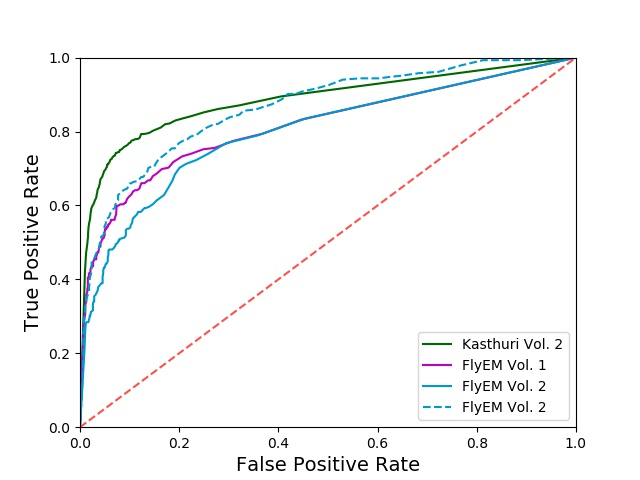
\includegraphics[width=0.45\linewidth]{./figures/receiver-operating-characteristic.jpg}
	\caption{The receiver operating characteristic (ROC) curves of our classifier on three connectomics datasets. The classifier works best on previously unseen data of the Kasthuri volume. The dashed blue line indicates better performance on the FlyEM datasets with retraining compared to without (solid blue).}
	\label{fig:receiver-operating-characteristic}
\end{figure}

\paragraph{Neural Network Transference.}
\TODO{rename: Generalization to Other Dataset.}
Our neural network does not take as input the images or affinities to allow us to transfer network weights from one dataset to the next.
Table~TODO{X} shows the result when training on the FlyEM data and inferring on the Kasthuri data and vice versa.
The classification results are reasonable despite the fact that the datasets vary in resolution and even animal type.


\subsection{Graph Optimization Results}

The graph optimization strategy using multicut increases our accuracy over using just the CNN.
Table \ref{table:multicut} shows the changes in precision, recall, and accuracy for all four datasets compared to the CNN.
The precision increases on each dataset, although the recall decreases on all but one of the datasets.Since it is more difficult to correct merge errors than split errors, it is often desirable to sacrifice recall for precision.
Over the three testing datasets, applying a graph-based partitioning strategy reduced the number of merge errors by \TODO{XX}\%, \TODO{XX}\% and \TODO{XX}\%, respectively. 

\begin{table}[h]
	\centering
	\small
	\begin{tabular}{c c c c} \hline
		\textbf{Dataset} & $\Delta$ \textbf{Precision} & $\Delta$ \textbf{Recall} & $\Delta$ \textbf{Accuracy} \\ \hline
		Kasthuri Training & +3.61\% & -0.53\% & +0.60\% \\
		Kasthuri Vol. 2 & +7.59\% & -1.77\% & +1.38\% \\
		FlyEM Vol. 1 & +2.68\% & +0.76\% & +0.66\% \\
		FlyEM Vol. 2 & +2.22\% & -1.05\% & +0.29\% \\ \hline
	\end{tabular}
	\caption{Precision, recall, and accuracy changes between CNN only and CNN paired with graph-optimized reconstructions for the training and three test datasets. The combined method results in better precision and accuracy.}
	\label{table:multicut}
\end{table}

\TODO{How does using lifted-multicut improve the results!}

\TODO{What are the benefits of post processing?}